%Toy example text
For illustrative purposes, we choose a simple linear system (point mass dynamics) to first illustrate our method. The point-mass system has the following dynamics:
\begin{equation}
\label{eq:PointMass}
x_{k+1} = x_k + u_k
\end{equation}
The control problem we solve is a generalized version of \eqref{eq:min rob problem} (using the smooth version of robustness), given by
\begin{subequations}
\label{eq:general_ctrl}
\begin{align}
\text{max } & \srob_{\Psi}(\sstraj) - \gamma \sum_{k=0}^{N-1} l(x_{k+1},u_{k}) \\
\text{s.t. } & x_{k+1} = f(x_k,u_k), \, \forall k=0,\dotsc,N-1 \\
 & x_k \in X, \, \forall k=0,\dotsc,N \\
 & u_k \in U, \, \forall k=0,\dotsc,N-1 \\
 & \delta \srob_{\Psi}(\sstraj) \geq 0
\end{align}
\end{subequations}

If we set $\gamma=0$ and $\delta=0$, we recover the problem in \eqref{eq:min rob problem}. In the above formulation, $l(x_{k+1},u_{k})$ is a system specific control cost, e.g. the LQR cost $x_k'Qx_k + u_k'Ru_k$. $X$ and $U$ define constraints on the state $x$ and control $u$ respectively. 

For the point-mass example, we define the specification to be followed as $\Psi = \always_{[0,20]} \neg (x_k \in \text{Unsafe}) \land \eventually_{[0,20]} (x_k \in \text{Terminal})$, with the sets $\text{Unsafe}=[-1,1]^2$ and $\text{Terminal}=[2,2.5]^2$. In addition, for the control problem, $X=[-2.5,2.5]^2$, $U=[0.3,0.3]^2$, $\delta=1$, and we optimize for two different values of $\gamma$, $0.1$ and $0.001$, and start with an initial point $x_0=[-2,-2]'$. The control cost is $l(x_k) = ||x_k||_{2}^2$, which when summed over is the square of the trajectory length. Note, $N=20$, which is the horizon length of the specification.

An initial trajectory starting from $x_0$ and ending in the $\text{Terminal}$ set is obtained via solving a linear program for feasibility ($\text{minimize } 0$) with the system dynamics and input/state constraints, and the terminal set added as a constraint. This trajectory is used to initialize the SQP optimization.

Fig.\ref{fig:toy control} shows the sets, initial trajectory (which is unsafe and has a robustness of $-1$), and the two trajectories for the two values of $\gamma$. Both trajectories satisfy the specification $\Psi$. Intuitively, the trajectories in Fig.\ref{fig:toy control} make sense, as for a higher value of $\gamma=0.1$ we get a shorter trajectory, which is closer to unsafe set, hence satisfies $\Psi$ less robustly ($\rob_{\Psi}=0.6543)$) and for a smaller value of $\gamma=0.001$ we get a longer trajectory which has a higher robustness ($\rob_{\Psi}=1.2073)$).

\begin{figure}[t]
\centering
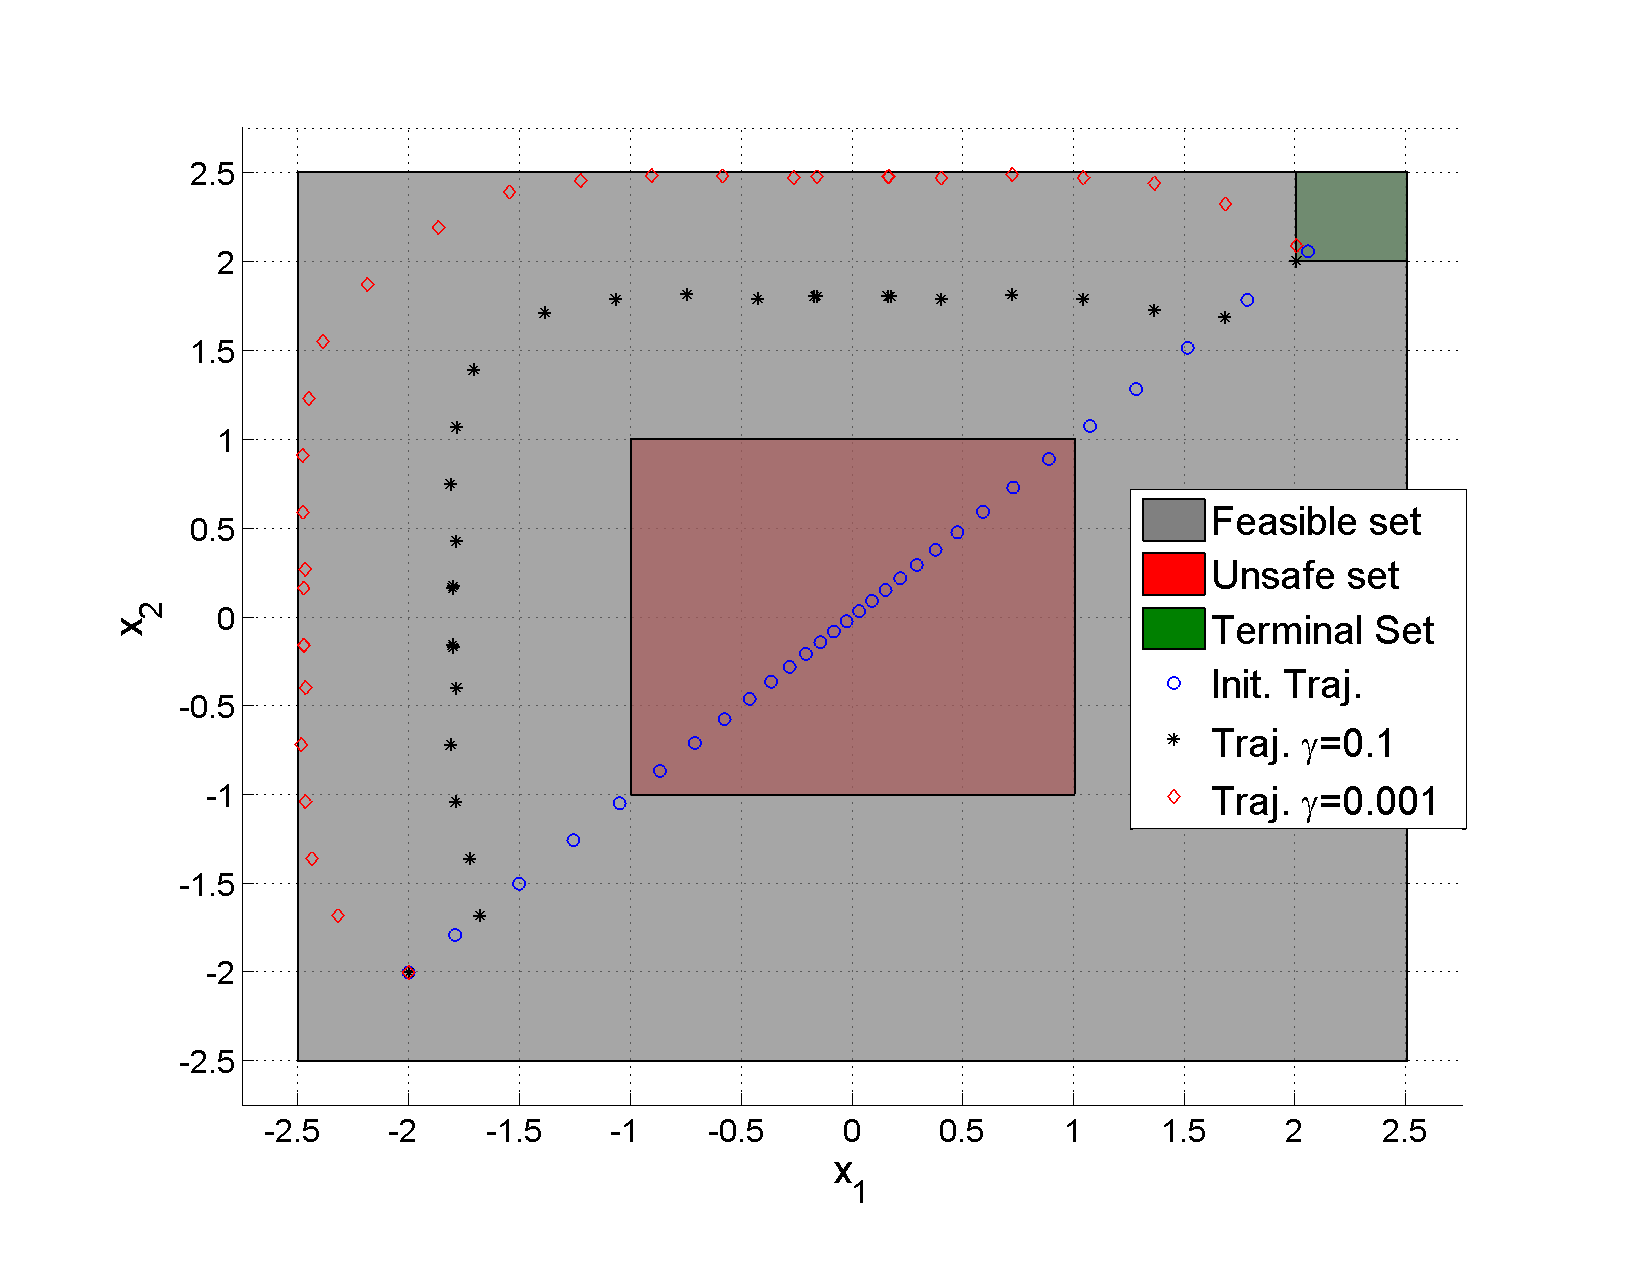
\includegraphics[width=0.49\textwidth]{figures/ToyExampleControl}
\caption{Initial trajectory and trajectories obtained for two different values of $\gamma$ in \eqref{eq:general_ctrl}.}
\label{fig:toy control}
\end{figure}